\documentclass[11pt,a4paper]{report}

%
% Packages
%
\usepackage[T1]{fontenc}
\usepackage[utf8]{inputenc}
\usepackage{amsmath,amsthm,amssymb}
\usepackage[svgnames]{xcolor}
\usepackage[english,french]{babel}
\usepackage{multicol}
\usepackage{pstricks,pst-node,pst-text,pst-poly,pst-3d}
\usepackage{enumitem}
\usepackage{sidenotes}
\usepackage{graphicx} % Required to insert images
\usepackage{array}
\usepackage{booktabs} % Required for better horizontal rules in tables


%
% Constant and Variables
%
\setlength{\textwidth}{175mm}
\setlength{\textheight}{255mm}
\setlength{\oddsidemargin}{-10mm}
\setlength{\topmargin}{-15mm}
\setlength{\parskip}{0.2cm}

\definecolor{vertfonce}{rgb}{0,0.5,0}

%
% Commands
%
\newcommand{\ds}{\displaystyle}
\newcommand{\scr}{\scriptscriptstyle}
\newcommand{\bs}[1]{\ensuremath{\boldsymbol{#1}}}
\renewcommand{\leq}{\leqslant}
\newenvironment{refer} 
{
	\begin{list}
		{}
		{
			\setlength{\labelwidth}{.5em}
			\setlength{\leftmargin}{0.4cm}
			\setlength{\itemsep}{0cm}
		} 
	}
	{\end{list}}
%\pagenumbering{roman}
%\setcounter{page}{1}

%
\newcounter{num}
\newcommand{\exo}{\addtocounter{num}{1}\noindent{\bf{Exercice \thenum}}\\[-1mm]}
%

%
\newcommand{\donnee}[1]{\\{Donnée: } \emph{#1}}
%


%
% Math
%
\newcommand{\Real}{\mathbb R}
\newcommand{\RPlus}{\Real^{+}}
\newcommand{\norm}[1]{\left\Vert#1\right\Vert}
\newcommand{\abs}[1]{\left\vert#1\right\vert}
\newcommand{\setn}[1]{\left\{#1\right\}_{\scriptscriptstyle n \ge 1}}
\newcommand{\set}[1]{\left\{#1\right\}}
\newcommand{\seq}[1]{\left<#1\right>}
\newcommand{\eps}{\varepsilon}
\newcommand{\To}{\longrightarrow}
\newcommand{\Prob}{\rm{P}}
\newcommand{\F}{\mathcal{F}}
\newcommand{\h}{\mathcal{H}}
\newcommand{\M}{\mathcal{M}}
\newcommand{\N}{\mathcal{N}}
\newcommand{\E}{{\rm E}}
\newcommand{\Hnull}{{\rm H}_{0}}
\newcommand{\Hone}{{\rm H}_{1}}
\newcommand{\Var}{{\rm Var}}
\newcommand{\Cov}{{\rm Cov}}
\newcommand{\sign}{{\rm sign}}
\newcommand{\med}{{\rm med}}
\newcommand{\tr}{{\rm tr}}
\newcommand{\T}{{\text{\tiny \rm T}}}
\newcommand{\minf}{- \, \infty}
\newcommand{\intervalle}[4]{\mathopen{#1}#2\mathpunct{},#3\mathclose{#4}}
\newcommand{\intervalleff}[2]{\intervalle{[}{#1}{#2}{]}}
\newcommand{\intervalleof}[2]{\intervalle{]}{#1}{#2}{]}}
\newcommand{\intervallefo}[2]{\intervalle{[}{#1}{#2}{[}}
\newcommand{\intervalleoo}[2]{\intervalle{]}{#1}{#2}{[}}   
%
\newcommand{\separation}{{\begin{center}\rule{10cm}{0.25pt}\end{center}}\noindent}
%
\frenchspacing


\begin{document}
	\header{probabilités conditionnelles et indépendance}{Série 2}
	%
	% Exercice 1
	%
	\begin{exo}
		\donnee{À vue d’oeil, il fait beau sept fois sur dix à Yverdon–les–Bains le jour de la rentrée académique. Votre enseignant de probabilités et statistique dispose de deux sources de prévisions météorologiques indépendantes: le service météorologique suisse qui se trompe deux fois sur cent et une grenouille verte, qui se trompe une fois sur vingt.}
		\begin{subexo}{À l’aide de l’énoncé, donner les probabilités}
			\begin{multicols}{4}
				\begin{enumerate}
					\item	$P(F|E)$
					\item	$P(F|\conj{E})$
					\item	$P(G|E)$
					\item	$P(G|\conj{E})$
				\end{enumerate}
			\end{multicols}
		\end{subexo}
		\begin{subexo}{Calculez les probabilités}
			\begin{multicols}{2}
				\begin{enumerate}
					\item $P(\conj{F}\cap G|E)$
					\item $P(\conj{F}\cap G|\conj{E})$
				\end{enumerate}
			\end{multicols}
		\end{subexo}
	\end{exo}
	
	%
	% Exercice 2
	%
	\begin{exo}
		\donnee{Pour éviter un incendie, une alarme a été installée dans la cuisine d’un restaurant australien.Supposons que la probabilité que l’alarme retentisse par erreur un jour donné sans qu’il y ait incendie est 0.01 et celle qu’elle retentisse en cas d’incendie vaut 0.95. De plus, on suppose que la probabilité qu’un incendie se déclare dans la cuisine un jour donné est 0.005}
		\begin{subexo}{	Calculer la probabilité que l'alarme retentisse un jour donné.}
			sdaf
		\end{subexo}
		\begin{subexo}{		Déterminer la probabilité qu'un incendie se déclare dans la cuisine un jour donné en sachant que l'alarme l'a signalé.}
			adsf
		\end{subexo}
	\end{exo}
	
	%
	% Exercice 3
	%
	\begin{exo}
		\donnee{Un signal binaire valant 0 ou 1 est envoyé par câble électrique. La transmission est affectée par des perturbations dites “bruits” : le signal 0 est reçu en 1 avec probabilité 0.2 et le signal 1 est enregistré en 0 avec probabilité 0.1. Définissons les événements suivants:
		\\ $E_0$ : "le signal émis vaut 0"
		\\ $E_1$ : "le signal émis vaut 1"
		\\ $R_0$ : "le signal reçu vaut 0"
		\\ $R_1$ : "le signal reçu vaut 1" 
		\\En supposant que le système de transmission émet le signal 0 avec probabilité 0.45, calculer les probabilités de transmission correctes }
		\begin{subexo}{$P(E_0 | R_0)$}
			sdaf
		\end{subexo}
		\begin{subexo}{$P(E_1 | R_1)$}
			sdaf
		\end{subexo}
	\end{exo}
	%
	% Exercice 4
	%
	\begin{exo}
		\donnee{On jette de suite deux dés équilibrés. Considérons les événements :
			\\• A : “la somme des faces vaut 6”;
			\\• B : “le premier dé donne 4”;
			\\• C : “la somme des faces vaut 7”.
			Les événements A et B sont-ils indépendants ? Qu’en est-il des événements B et C ? Donnez une interprétation intuitive des résultats.}
		\begin{subexo}{Les événements A et B sont-ils indépendants ? Qu’en est-il des événements B et C ? Donnez une interprétation intuitive des résultats.}
		\end{subexo}
	\end{exo}
	%
	% Exercice 5
	%
	\begin{exo}
		\donnee{Un système électronique est formé des composants A, B, C et D placés selon le dispositif de la Figure 1. On suppose que les composants fonctionnent indépendamment les uns des autres et leurs probabilités de fonctionnement sont toutes égales à 0.8. Le système est opérationnel s’il existe un chemin entre les points I et O ne comprenant que des composants qui fonctionnent. Calculer la probabilité que le système soit défaillant.\\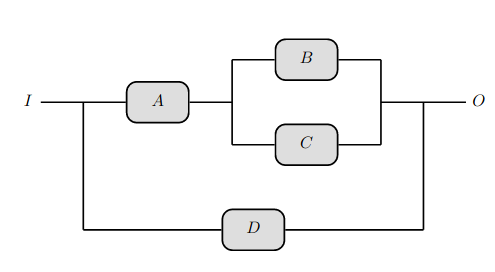
\includegraphics[width=10cm]{ex5.png}}
	\end{exo}
	%
	% Exercice 6
	%
	\begin{exo}
		\donnee{La société Gloup s’intéresse à la capacité de détection que possède le filtre bayesien anti-spam qu’elle vient d’installer. Dans la liste des mots et symboles permettant de détecter des messages publicitaires figurent les mots “viagra” et “miracle”. Par simplification, notons ces mots 1 et 2 et les probabilités:
			\\\indent$p_i$ : probabilité qu’un mot choisi au hasard dans un message électronique est le mot i en sachant que le message est un spam
			\\\indent$q_i$ : probabilité qu'un mot choisi au hasard dans un message électronique est le mot i en sachant que le message n’est pas un spam
			\\valent respectivement $p_1$ = 0.05, $p_2$ = 0.1 et $q_1$ = 0.001, $q_2$ = 0.5. Supposons que dans chaque type de messages électroniques, les mots de la liste se trouvent indépendamment les uns des autres dans les messages. La proportion de messages spam reçus par la société Gloup vaut 0.9. En sachant que les mots “viagra” et “miracle” figurent tous les deux une fois dans le même message électronique, déterminer la probabilité qu’il s’agisse d’un spam.}
	\end{exo}
	%
	% Exercice 7
	%
	\begin{exo}
		\donnee{En sachant que pour le jour de la rentrée académique, la météo avait annoncé de la pluie le matin alors que le comportement de la grenouille avait laissé présager du soleil, calculer la probabilité qu'il allait faire beau à Yverdon le matin de la rentrée.}
	\end{exo}
	%
	% Footer
	%
	\vfill
	\hrule
	\vspace{2mm}
	\noindent {\tiny Corrigé Etudiant - TIC} \hfill {\tt \tiny \today}
\end{document}
